The results in 1D are very promising, but the real open challenges are situated in 2 (or higher) dimensions. Therefore, it is an interesting and relevant question whether the results generalise to 2D. These results are twofold. On the one hand, a similar measure as in 1D is calculated to measure how good a method works on a specific 2D grid. Here, we will need to settle for what can be computed. As a second measure, and from physical point of view the most interesting one, some phase transitions of the 2D transveral Ising model are determined, and compared against values in literature.

\subsection{Norm}

Once again, a suitable norm has to be derived. The situation is more difficult than in 1D, because contracting a PEPO tensor network has a much larger computational complexity than in 1D. Ideally, the norm would be calculated on a nxn cyclical grid (2D grid on a torus). Here n has to be at least 1 larger than the largest explicitly constructed chain.

In practice, this is not achievable in reasonable amount of time. The limitations are twofold: the maximum number of sites to calclate the matrix exponential is still around 14, and the contraction of the tensor network is limited to \todo{number}

The limitations on the PEPO contraction can be somewhat relaxed by not computing the full network, but computing the reduced density matrix. Here, most of the sites have their physical indices traced out, except for one site.

The final error measures are defined by:
\begin{equation}\label{res2d:err_Def}
    \rho^1_{i,j} =\vcenter{ \hbox{ \pepob{8}{8}{{
                        "-","-", "-","-","-","-","-",
                        "",  "", "","","","","",
                        "",  "", "","","","","",
                        "",  "", "","","","","",
                        "",  "", "","","","","",
                        "",  "", "","","","","",
                        "",  "", "","","","","",
                        "-", "-", "-","-","-","-","",}}{{
                        "-","-", "-","-","-","-","-",
                        "","", "","","","","",
                        "","", "","","","","",
                        "","", "","","","","",
                        "","", "","","","","",
                        "","", "","","","","",
                        "","", "","","","","",
                        "-","-", "-","-","-","-","",}}{{
                        1,13,1,1,1,1,1,1,
                        1,0,1,1,1,1,1,1,
                        1,0,1,1,1,1,1,1,
                        1,0,1,1,1,1,1,1,
                        1,0,1,1,1,1,1,1,
                        1,0,0,0,1,1,1,1,
                        13,12,0,0,0,0,0,13,
                        1,13,1,1,1,1,1,1,
                    }} }}
\end{equation}
and
\begin{equation}\label{res2d:err_Def}
    \rho^2_{i,j} =\vcenter{ \hbox{ \pepob{8}{8}{{
                        "-","-", "-","-","-","-","-",
                        "",  "", "","","","","",
                        "",  "", "","","","","",
                        "",  "", "","","","","",
                        "",  "", "","","","","",
                        "",  "", "","","","","",
                        "",  "", "","","","","",
                        "-", "-", "-","-","-","-","",}}{{
                        "-","-", "-","-","-","-","-",
                        "","", "","","","","",
                        "","", "","","","","",
                        "","", "","","","","",
                        "","", "","","","","",
                        "","", "","","","","",
                        "","", "","","","","",
                        "-","-", "-","-","-","-","",}}{{
                        1,1,1,1,1,1,1,1,
                        1,1,1,1,1,1,1,1,
                        1,1,1,1,1,1,1,1,
                        1,1,1,1,1,1,1,1,
                        1,1,1,0,0,1,1,1,
                        1,0,0,12,0,0,0,1,
                        1,0,0,0,0,0,0,1,
                        1,1,1,1,1,1,1,1,
                    }} }}
\end{equation}
For the first one, all the blocks in the expansion are present in, and it is cyclical in both x and y. The second reduced density matrix is not cyclic, but includes more loop type contributions. Both relative errors will be used, defined by :
\begin{equation}
    \epsilon^{\alpha} = \frac{  {  \left \|  \rho^{\alpha}_{exact,  i,j}- \rho^{\alpha}_{ i,j}  \right \|} _{2}  }{ {  \left\|  \rho^{\alpha}_{exact,  i,j} \right \|}_2} \quad \alpha \in [1,2]
\end{equation}
For the given error measures, series expansion up till order 5 can be tested. The second norm takes the most time to compute, due to the larger complexity of contracting the tensor network.

\subsection{Models}

\subsubsection{Ising}

We first determine the optimal value $\sigma_0$ for pseudoinversion and test the influence of the addition of plaquette term to the expansions. The series is of order 5, and the transversal field is of magnitude 2.5.The results can be seen in \cref{ig:res2d:n1:tising}.

The truncation parameter $\sigma_0$ was optimal at a value of about $\sigma_0=10^{-12}$ in 1D. Smaller values resulted in divergent series exapnsions. In the graph we see that even better behaved inverses of $\sigma_0=10^{-10}$ improve upon the error made.

The plaquette term (\cref{tikzfig:plaquette}) is mainly important at low $\beta$ to keep the error low, and also has some considarable influence at higher temperatures.

\begin{figure}
    \center
    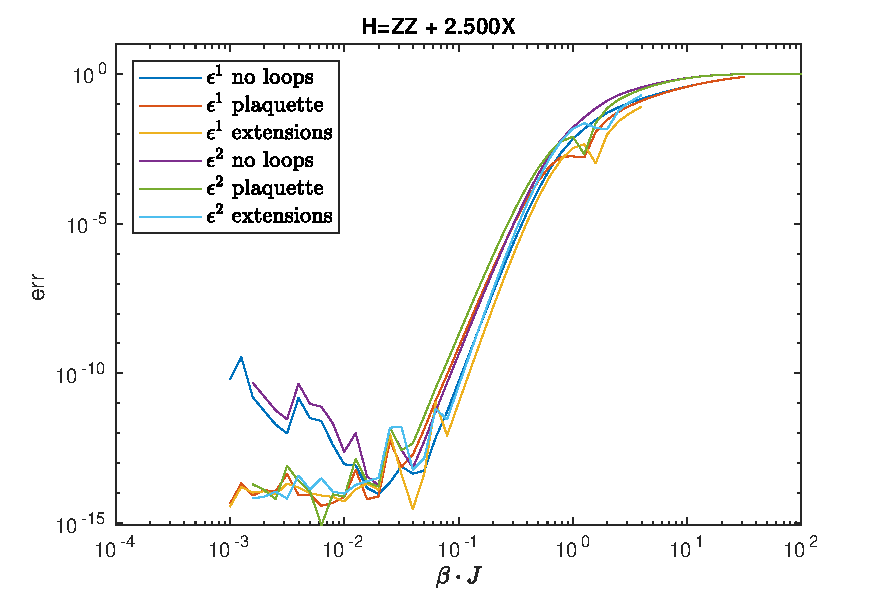
\includegraphics[width=\textwidth]{Figuren/benchmarking/2D_Err01_t_sing.pdf}
    \caption{ }
    \label{fig:res2d:n1:tising}
\end{figure}
\todo{fix caption}

\subsubsection{Heisenberg}

\subsection{Conclusion}
